\documentclass[10pt,xcolor=pdflatex]{beamer}
\usepackage{newcent}
\usepackage[utf8]{inputenc}
%\usepackage[czech]{babel}
\usepackage{biblatex}
\usepackage{hyperref}
\usepackage{fancyvrb}
\usepackage{tikz}
\usepackage{tikz-qtree}
\usepackage{float}
\usetheme{FIT}

\usetikzlibrary{arrows,backgrounds,shadows, positioning}
\bibliography{prezentace.bib}

\pgfdeclarelayer{edgelayer}
    \pgfdeclarelayer{nodelayer}
% tell TikZ how to stack them (back to front)
    \pgfsetlayers{nodelayer,main,edgelayer}

%%%%%%%%%%%%%%%%%%%%%%%%%%%%%%%%%%%%%%%%%%%%%%%%%%%%%%%%%%%%%%%%%%
\title[strace2seccomp]{Automatic Seccomp Syscall\\Policy Generator}

\author[]{Marek Tamaskovic}

\institute[]{Brno University of Technology, Faculty of Information Technology\\
Bo\v{z}et\v{e}chova 1/2. 612 66 Brno - Kr\'alovo Pole\\
xtamas01@fit.vutbr.cz}

\date{August 22, 2018}
%\date{\today}
%\date{} % bez data

%%%%%%%%%%%%%%%%%%%%%%%%%%%%%%%%%%%%%%%%%%%%%%%%%%%%%%%%%%%%%%%%%%

\begin{document}

\frame[plain]{\titlepage}

\begin{frame}\frametitle{Introduction}

\begin{columns}
  \begin{column}{0.6\textwidth}
     \begin{itemize}
       \item Ing. Lenka Turo\v{n}ov\'a
       \item Bc. Daniel Kope\v{c}ek
       \item Cooperation with RedHat Inc.\\
       \item Motivation?
     \end{itemize}
  \end{column}
  \begin{column}{0.4\textwidth}
      \begin{center}
        \includegraphics[width=1\textwidth]{img/Logo_RH_BW_RGB}
      \end{center}
  \end{column}
\end{columns}

\end{frame}

\begin{frame}\frametitle{Input / Output}
    \begin{columns}
        \begin{column}{0.5\textwidth}
          Input:
          \begin{itemize}
            \item \emph{strace} log
          \end{itemize}
        \end{column}
        \begin{column}{0.5\textwidth}
          Output:
          \begin{itemize}
            \item C\textbackslash C++ code template
            \item \emph{libseccomp}
          \end{itemize}
        \end{column}
    \end{columns}
\end{frame}

\begin{frame}\frametitle{Architecture}
  \begin{figure}[h]
  \centering
  \resizebox {\textwidth} {!} {
    \input{../obrazky-figures/architecture0}
  }
  % \caption{Architecture of strace2seccomp}
  \label{fig:tikz:architecture}
\end{figure}
\end{frame}

\begin{frame}\frametitle{Optimiziations}

  \begin{itemize}
    \item Three optimization levels
     \begin{itemize}
	    \item \emph{Strict}:
	    \begin{itemize}
	      \item 1:1
	      \item input $\rightarrow$ output
	    \end{itemize}
	    \item \emph{MinMax}:
	    \begin{itemize}
	      \item allowed intervals
	      \item border values are extremes
	    \end{itemize}
	    \item \emph{DBSCAN}\footnote{Density-based spatial clustering of applications with noise}:
	    \begin{itemize}
	      \item implemented DBSCAN\cite{Mahesh_Kumar2016, Schubert:2017:DRR:3129336.3068335}
	    \end{itemize}
	  \end{itemize}
  \end{itemize}

 
\end{frame}

\begin{frame}\frametitle{What have I achieved?}
    \begin{itemize}
    	\item Designed program architecture
    	\item Implemented:
    	\begin{itemize}
    		\item \emph{IDS}\footnote{Intermediate Data Structure}
    		\item 3 algorithms
    	\end{itemize}
    	\item Created \emph{testsuite}
    	\item \textit{"It is on good way to appear in production"}
    \end{itemize}
\end{frame}

\begin{frame}\frametitle{Planed Extensions}
  \begin{itemize}
    \item \emph{Go} support
    \item \emph{ASLR}\footnote{Address Space Layout Randomization} turned off
    \item Customizable template
    \item Packaging
    \item More algorithms
  \end{itemize}
\end{frame}

\begin{frame}[allowframebreaks]
	\frametitle{References}
	\printbibliography
\end{frame}

\bluepage{Any questions?}

\appendix

\begin{frame}\frametitle{Question for defense}
    Název vašeho algoritmu je Minmax nebo Minimax? (V BP je toto nekonzistentní, i ve zdrojových kódech). Dokážete vysvětlit rozdíl oproti existujícímu algoritmu Minimax?
\end{frame}

\begin{frame}\frametitle{Inner Representation}
  \begin{figure}[h]
  \centering
  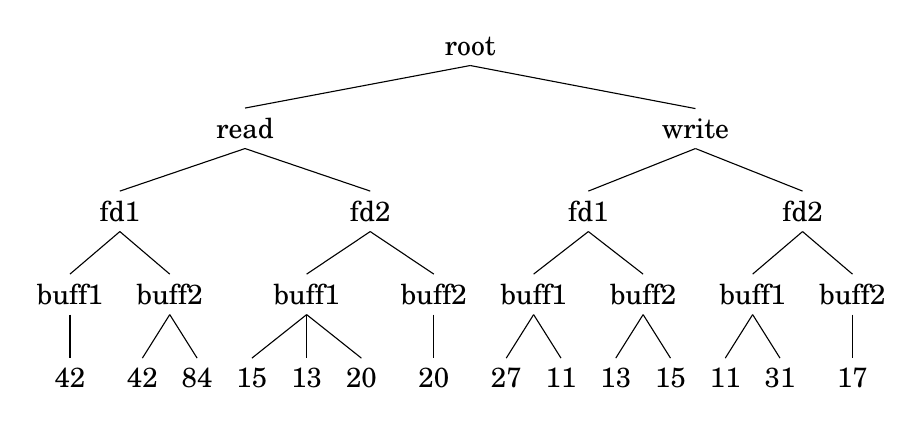
\begin{tikzpicture}
  \Tree [.root
          [.read
            [.fd1
              [.buff1 42 ]
              [.buff2 42 84 ]
            ]
            [.fd2
              [.buff1 15 13 20 ]
              [.buff2 20 ]
            ]
          ]
          [.write
            [.fd1
              [.buff1 27 11 ]
              [.buff2 13 15 ]
            ]
            [.fd2
              [.buff1 11 31 ]
              [.buff2 17 ]
            ]
          ]
        ]
  \end{tikzpicture}
  % \caption{Visualized IDS as a tree}
  \label{fig:tikz:IDStree}
\end{figure}
\end{frame}

\end{document}
